%%%%%%%%%%%%%%%%%%%%
% Header Stuff
%%%%%%%%%%%%%%%%%%%%
\documentclass[12pt]{article}
\usepackage[utf8]{inputenc}
\usepackage{setspace,graphicx,multirow,cite,caption}
\graphicspath{{figures/}}
\bibliographystyle{plain}

% Title/Sections Package
\usepackage{titlesec}
\titleformat*{\section}{\normalsize\bfseries}
\titleformat*{\subsection}{\normalsize\bfseries}
\titleformat*{\subsubsection}{\normalsize\bfseries}
\titleformat*{\paragraph}{\normalsize\itshape}
\titleformat*{\subparagraph}{\normalsize\itshape}
\titlespacing*{\section}{0pt}{1em}{0pt}
\titlespacing*{\subsection}{0pt}{1em}{0pt}
\titlespacing*{\subsubsection}{0pt}{1em}{0pt}

% Linguistics Packages
\usepackage{tikz,tikz-qtree,enumitem,float}
\usepackage[linguistics]{forest}
\usepackage{gb4e}
\tikzset{
  treenode/.style = {shape=rectangle, rounded corners,
                     draw, align=center,
                     top color=white, bottom color=blue!20},
  root/.style     = {treenode, font=\Large, bottom color=red!30},
  env/.style      = {treenode, font=\ttfamily\normalsize},
  dummy/.style    = {circle,draw}
}

% Title
\title{{\normalsize\bfseries {Structural Prediction in Online Processing: \\ \small{Binomial Each \& Wh-Moved Reflexives}}}}
\author{\normalsize\bfseries {Devin Johnson}}
\date{}


%%%%%%%%%%%%%%%%%%%%
% Main Document
%%%%%%%%%%%%%%%%%%%%
\begin{document}

\maketitle

\section{Introduction}
This paper is concerned with structural prediction in online sentence processing. In general, prediction
can be used to refer to any behavior by the parser in which hypotheses are generated concerning
(unseen) upcoming material based on information in the left-context \cite{Crocker2002,Kazanina2017}.
We take the term structural to mean that the hypotheses generated by the parser contain information
about the hierarchical relations the upcoming (predicted) element is subject to. Though there has been interest in structural prediction, there are (to our knowledge) relatively few studies which have provided strong evidence for the parser exhibiting such behavior \cite{Yoshida-Dickey-Sturt2013,Staub-Clifton2006, Kazanina2017, Phillips2006}.

As noted by previous reviews \cite{Kutas-DeLong-Smith2011,Kamide2008}, a problem for studies in structural prediction is that many results on the topic are often also interpretable via integration \cite{Kutas-Hillyard1980} theories.
The main distinction we draw between prediction and integration is in the directionality of processing; In prediction, upon encountering an element which the parser knows is subject to some dependency, it launches a subprocess to predict the other element(s) of the dependency in the upcoming input. In integration, upon encountering each element, the parser must integrate (i.e., insert, fit) it in with the preceding context. The ease of this integration may be explained via cue-retrieval (cite), feature matching, etc. Regardless of explanation, any effects on the current element would be viewed as a consequence of the ease in which it can be integrated, which is ultimately based on factors relevant to the preceding input. 

Let us illustrate how integration and prediction effects can be confused with a simplified example. Consider the production rules and the following sentence which the parser is tasked with:
\begin{exe}
    \ex
    \begin{xlist}
        \ex $AuxP \rightarrow [Aux \hspace{0.1cm} VP]$
        \ex $VP \rightarrow V'$
        \ex $ V' \rightarrow  [(Adv) \hspace{0.1cm} V]$
        \ex $V'\rightarrow [V \hspace{0.1cm} NP]$
    \end{xlist}
\end{exe}
``He has (really) (never) (...) gone to Europe.''\\

\noindent
In the example above, a predictive view might hypothesize that the perfective aux \textit{has} triggers a prediction of an upcoming past-participle V. So, upon encountering a past-participle V, the prediction results in facilitation at its position. However, under an \textit{integration} view we might hypothesize that upon reaching the past-participle V \textit{gone}, we must integrate. Since a past-participle is more predictable (*not* predicted) given the preceding aux, we should receive a facilitation at its position. The main issue is that the \textit{same effects} are expected to occur at the \textit{same place} in the input. Overall this shows the difficulty of distinguishing structural predictive theories from integration theories. Our main goal in this paper is to contribute new findings on the topic which are not easily interpretable by integration. To do so, we will present the results of two experiments on previously-untested structural configurations including binomial each \cite{Boeckx-Hornstein2005,Safir-Stowell1987,Burzio1986} and wh-moved reflexives.

\section{Past Work}
Recall that we see structural prediction as the phenomenon where hypotheses generated by the parser contain information about the hierarchical relations the upcoming (predicted) element is subject to. In addition, we distinguish prediction from integration via the direction of processing, as explained in the introduction. In the following, we present findings which we believe have shown convincing evidence for the parser performing structural prediction. Importantly, we believe these findings succeed at distinguishing structural prediction from integration. In our study, we build on these previous findings by testing more structural configurations.

\subsection{Phillips (2006)}
Philips (2006) \cite{Phillips2006} demonstrated evidence for structural prediction in the case of parasitic gap constructions \cite{Engdahl1983}. Parasitic gapping is a unique variant of wh-filler-gap dependency featuring two gaps, one independent and one depedent. While the independent gap can stand alone, the dependent (parasitic) gap needs the presence of the independent gap to be acceptable. An example adopted from Phillips (2006) is provided below:
\begin{exe}
    \ex
    \begin{xlist}
        \ex *What did the attempt to repair \_\_\__{gap.bad} ultimately damage the car?
        \ex What did the attempt to repair the car ultimately damage \_\_\__{gap.good}?
        \ex What did the attempt to repair \_\_\__{gap.p} ultimately damage \_\_\__{gap.good}?
    \end{xlist}
\end{exe}

\noindent
Parasitic gaps are known to be illicit when occurring in tensed (finite) subject NPs. Phillips
confirmed this with acceptability ratings and devised items such as those below:
\begin{exe}
    \ex
    \begin{xlist}
        \ex The outspoken environmentalist worked to investigate what the local campaign to preserve \_\_\__{gap.p} had harmed \_\_\__{gap.good}.
        \ex *The outspoken environmentalist worked to investigate what the local campaign that preserved \_\_\__{gap.p} had harmed \_\_\__{gap.good}.
    \end{xlist}
    \label{ex:gaps2}
\end{exe}
With this in mind, Phillips posited that upon reaching the parasitic gap in \ref{ex:gaps2}a, the parser is aware that a second, independent gap must be upcoming to license it. However, the parser does not know where this gap will occur. Philips found that reading times were longer on the verb \textit{preserve(d)} in the infinitival context \ref{ex:gaps2}a than they were in the finite context \ref{ex:gaps2}b. Phillips claimed that the increased reading time in the infinitival case suggests that the parser attempts to posit a gap in that location. Conversely, where a parasitic gap was not possible in \ref{ex:gaps2}b, no slowdown was detected, suggesting that no gap was posited.

The key claim is that, in order to show this behavior, the parser would need information about the structure in which the first (parasitic) gap occurs and make a prediction that upcoming licensing gap will occur. Philips (2006) argued that the only source of information that could lead to this prediction is top-down syntactic constraints. We believe that this study shows promising evidence for structural prediction. In addition, if we attempt to explain these results via integration, it is difficult to understand the slowdown at the possible gap location. For example, if we claim that the infinitive \textit{to preserve} is more difficult to integrate and therefore more slowly read, then how/why is this the case?

\subsection{Yoshida, Dickey, Sturt (2013)}
Yoshida, Dickey and Sturt (2013) \cite{Yoshida-Dickey-Sturt2013} showed sentences with an elliptical construction where an embedded wh-phrase introduces a missing clause (\ref{ex:masaya1}). At the point of the wh, the sentence could conclude with the same (matching) interpretation of the previous clause (``...stories about himself he told'') or another clause entirely. To test if the parser predictively builds structure for a matching interpretation, they showed participants sentences with a preceding gendered name which either matched a reflexive in the wh phrase or not.
\begin{exe}
    \ex \textbf{\{John,Mary\}} told a lot of stories, but I don't know how many stories about \textbf{\{himself,herself\}} he was frustrated with.        
    \label{ex:masaya1}
\end{exe}
They hypothesized that if the parser builds the matching interpretation structure predictively, there would be a gender mismatch effect at the reflexive due to an incorrect antecedent in the prediction. Yoshida, Dickey and Sturt indeed found longer reading times when the gender mismatched with the name but only in the elliptical conditions - not controls without ellipsis. This, they claimed, shows that potential antecedents are only considered when there is hierarchical structure which will permit the reflexive to be grammatically related to the potential antecedent.

\section{Experiment 1: Prediction with Binomial Each}
\subsection{Background}
Studies of binomial each (BE) \cite{Burzio1986,Safir-Stowell1987,Boeckx-Hornstein2005}
have revealed that it typically attaches to the right end of an indefinite NP (e.g., one book \textit{each})
and requires an antecedent which must be a plural NP, such as in \ref{ex:be1}.
\begin{exe}
    \ex \label{ex:be1}
    \begin{xlist}
        \ex The \textbf{students} will read three books each for the final paper.
        \ex *The \textbf{student} will read three books each for the final paper.
    \end{xlist}
\end{exe}

\noindent
Furthermore, like reflexives, the position of BE must be c-commanded by its antecedent as in \ref{ex:be2}a. In
unacceptable \ref{ex:be2}b, the only possible plural NP antecedent, \textit{the men}, is embedded within an adjunct PP
and as such does not c-command the BE.
\begin{exe}
    \ex \label{ex:be2}
    \begin{xlist}
        \ex The teachers talked beside the \textbf{man} about three students each.
        \ex *The teacher talked beside the \textbf{men} about three students each.
    \end{xlist}

\end{exe}

\noindent
Combining the two points above, in wh-moved constructions, BE can form a dependency with an embedded subject so long as the embedded subject is a plural NP which c-commands the resulting gap. With this, we can construct sentences such as those in \ref{ex:be3}. In \ref{ex:be3}b, unacceptability can be explained by plural \textit{the men} not c-commanding $t_i$.
\begin{exe}
    \ex \label{ex:be3}
    \begin{xlist}
        \ex How many students each did the teachers talk beside the man about?
        \ex *How many students each did the teacher talk beside the men about?
    \end{xlist}
\end{exe}

\subsection{Participants}
173 native speakers of English were recruited through Prolific and participated in an online l-maze \cite{Forster-Guerrera-Elliot2009} experiment run on the PCIbex platform \cite{Zehr-Schwarz2018}. Completing the experiment took approximately 30-60 minutes total, and participants were compensated \$9 per hour.

\subsection{Design}
Considering what is known of BE, we created a 24-item, 2x2 factorial l-maze reading experiment in which we manipulated the usage of BE (factor 1) and the auxiliary (factor 2) preceding the matrix subject. The setup an example item is shown in Figure \ref{setupexp1}. In the control conditions without BE, sentence lengths were made to match by the insertion of an adjective prior to the first noun. In this way, we can remove what we see as the trigger of the predictive chain while still preserving the position of the target region (the auxiliary) for later analysis.
Participants were instructed to build sentences one word at a time by picking the most natural next word from two options per individual screen and considering preceding context of the sentence (not shown). In the l-maze paradigm, each screen contains the desired (real) word and one pseudoword. If the participant selected the correct word, they continued building the sentence. Conversely, if the participant selected the pseudoword, they failed the sentence and moved to the next one. Participants continued building sentences until completing a total of 96 (24 target items, 72 distractors items).

\begin{figure}[h!]
    \centering
    \begin{tabular}{cll}
    \textbf{Binomial Each}                & \multicolumn{1}{c}{\textbf{x}} & \multicolumn{1}{c}{\textbf{Aux}}   \\
    $\in$                         &                       & \multicolumn{1}{c}{$\in$} \\
    \{BE, !BE\}                 &                       & \{Do, Does\}              \\
    \multicolumn{1}{l}{\textbf{}} &                       &                          
    \end{tabular}
    \begin{itemize}[label={}]
        \item \textbf{BE/Do} \\ How many printers \textbf{\{each\}_A}, according to the boss, \textbf{\{do\}_C} the calm but distracted deliverers_B say that the customers receive on a typical day?
        \item \textbf{BE/Does} \\ How many printers \textbf{\{each\}_A}, according to the boss, \textbf{\{does\}_C} the calm but distracted deliverer_B say that the customers receive on a typical day?
        \item \textbf{!BE/Do} \\ How many efficient printers \textbf{\{ \}}, according to the boss, \textbf{\{do\}_C} the calm but distracted deliverers_B say that the customers receive on a typical day?
        \item \textbf{!BE/Does} \\ How many efficient printers \textbf{\{ \}}, according to the boss, \textbf{\{does\}_C} the calm but distracted deliverer_B say that the customers receive on a typical day?
    \end{itemize} 
    \caption{Setup of Experiment 1. Factors, levels, and an example item.}
    \label{setupexp1}
\end{figure}

\subsection{Expected Results}
Let us explore the implications of a structurally predictive parser, referencing Figure \ref{fig:printers} below.
First, assuming the parser employs knowledge of the structural constraints of BE detailed above, the occurrence of BE (A) should lead to a prediction that a plural NP antecedent is upcoming in the first possible position - the matrix subject position (B). Once predicting the plural NP antecedent, given that it is in a structurally-dependent relation
with the morphology of the aux, the parser could further predict a plural aux (C). Thus, in the end, our theory should have us observe a facilitation effect at position C in BE/Do due to a correct prediction of plural aux. Conversely, we should observe an opposite (surprise) effect in BE/Does where the predictive chain results in an incorrect prediction (i.e., a plural aux). !BE/Do and !BE/Does function as controls and we do not expect a prediction.

In an integration theory, one possibility is that the always-plural NP inside the wh phrase (e.g. printers) primes the parser for a number-matching aux. If this is the case, \textit{do} should always integrate more easily, and we should see a facilitation in conditions containing \textit{do}, regardless of BE's presence. This would also predict a slowdown in conditions with the singular \textit{does} in all conditions containing it.

\begin{figure}[h!]
    \centering
    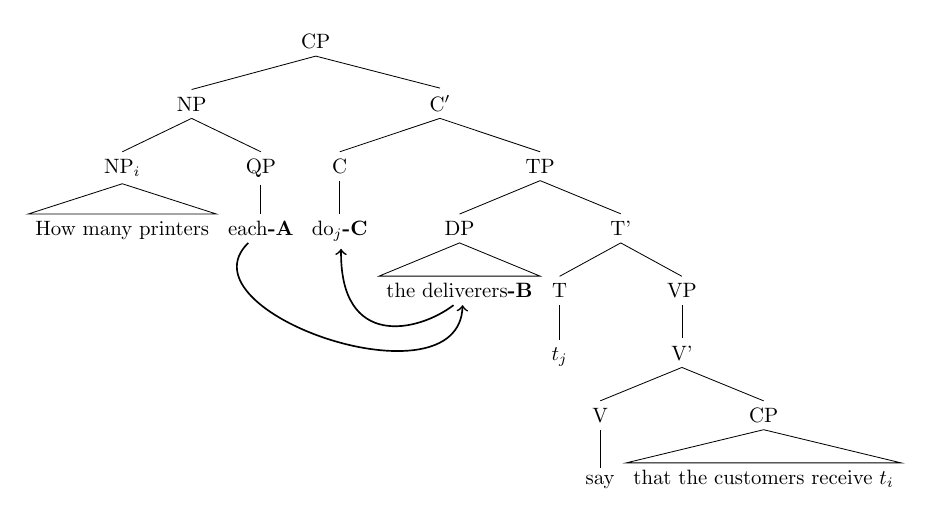
\begin{tikzpicture}[scale=0.75]
        \Tree [.CP [.NP [.NP$_i$ \edge[roof];\node(wh){How many printers}; ] [.QP \node(e){each\textbf{-A}};  ] ]
        [.C$'$ [.C \node(aux){do$_j$\textbf{-C}}; ]
        [.TP [.DP \edge[roof]; \node(subj){{the deliverers\textbf{-B}}}; ]  [.T' [.T \node(tense){$t_{j}$}; ] [.VP
        [.V' [.V say ] [.CP \edge[roof];\node(cp){that the customers receive $t_i$};  ] ]
        ] ] ] ] ]
        \draw[semithick,->] (e)..controls +(south west:2) and +(south:2)..(subj);
        \draw[semithick,->] (subj)..controls +(south west:1) and +(south:2)..(aux);
    \end{tikzpicture}
    \caption{Structural analysis of (abridged) BE/Do of
        Experiment 1. \textbf{A} is encountered first,
        which creates hypothesis chain A $\rightarrow$ B $\rightarrow$ C.
        Speedup or slowdown due to prediction is expected at position \textbf{C}.}
    \label{fig:printers}
\end{figure}

\subsection{Results}
Out of 188 participants, 15 were pruned from the dataset. Participants were removed if their total response accuracy was 50\% or lower and/or their mean reading time differed from the grand mean reading time by
more than two standard deviations. For each participant, wrong responses were removed due to the experiment
automatically moving to the next sentence upon an incorrect response. Additionally, reading times which were over two standard deviations from the mean (per participant, condition, and word number) were removed. Finally, an overall
reading time cutoff was used with a minimum of 300ms and a maximum of 3500ms.

Figure \ref{fig:howmanytarget} shows mean log reading times for each condition in the target region (position 9).
A significant main effect of auxiliary number was found ($\beta=-0.019$, $SE=0.004$, $t=-4.959$, $p < 0.0001$).
There was also a significant interaction effect observed ($\beta=0.007$, $SE=0.004$, $t=1.784$, $p=0.0745$). Subset pairwise comparison analysis revealed that BE/Does resulted in significantly
slower ($p < 0.0001$) reading times than BE/Do.

\begin{figure}[h!]
    \center
    \includegraphics[scale=0.50]{howmanytarget.png}
    \caption{Mean (log) reading times at critical region (do/does) across
        four conditions. Significant interaction effect and significant
        main effect on f2 (do/does).}
    \label{fig:howmanytarget}
\end{figure}

\subsection{Discussion}
Our design purposely separates the predictions of a structural prediction theory and an integration theory at the target position C. As expected, at the target region, significant slowing in reading time was found in BE/Does as compared to BE/Do. Although a main effect of aux number was found, it is important to note that !BE/Do and !BE/Does
(controls) did not differ significantly when aux number was manipulated. This is in line with our expectations because we do not expect any predictive process to occur without the presence of binomial each and thus no surprise or facilitation at the aux. These results rule out the an integration-based hypothesis based where slowdown/speedup is claimed to be due to the number (mis-)match of the wh NP (printers) and the aux.

Overall, it seems that BE indeed triggers the parser to posit an upcoming plural matrix subject. This in turn leads to a secondary prediction of an agreeing (plural) aux. Therefore, upon reaching a singular aux (contrary to the prediction) in BE/Does, we see a surprise effect. This lends support to the idea that the parser uses structural information about BE to predict part of the structural dependency. In addition, we have evidence that the parser can tie together information from multiple structural dependencies (ABC) to form a prediction. Although the computational implications will not be addressed in detail, if this is the case, it is an impressive feature which can serve to limit the space of possible parsers for any given grammar.

\section{Experiment 2: Prediction with Reflexives} 
\subsection{Background}
Past research has shown that anaphoric elements (reflexives, pronouns and ellipsis) must be c-commanded
by their antecedents \cite{Chomsky1981}. In addition, several sentence processing studies have shown that upon encountering an anaphoric element, the parser launches an active search for its antecedent \cite{Sturt2003,Kazanina-Lau-Lieberman-Yoshida-Phillips2007,Yoshida-Dickey-Sturt2013}.

\subsection{Participants}
88 native speakers of English were recruited through Prolific and participated in an online g-maze \cite{Forster-Guerrera-Elliot2009} experiment run on the PCIbex platform \cite{Zehr-Schwarz2018}. Completing the experiment took approximately 30-60 minutes total, and participants were compensated \$9 per hour.

\subsection{Design}
We created a 24-item, 2x2 factorial l-maze reading experiment in which we used a Wh-moved reflexive, manipulating the appearance of its antecedent and the plurality of a following aux. The setup an example item is shown in Figure \ref{setupexp1}.  Participants were instructed to build sentences one word at a time by picking the most natural next word from two options per individual screen and considering preceding context of the sentence (not shown). In the g-maze paradigm, each screen contains the desired (natural) word and one (real, but highly implausible) distractor word. If the participant selected the correct word, they continued building the sentence. Conversely, if the participant selected the pseudoword, they failed the sentence and moved to the next one. Participants continued building sentences until completing a total of 96 (24 target items, 72 distractors items).

\begin{figure}[h!]
    \centering
    \begin{tabular}{cll}
    \textbf{Antecedent}                & \multicolumn{1}{c}{\textbf{x}} & \multicolumn{1}{c}{\textbf{Aux}}   \\
    $\in$                         &                       & \multicolumn{1}{c}{$\in$} \\
    \{Ant, !Ant\}                 &                       & \{Does, Do\}              \\
    \multicolumn{1}{l}{\textbf{}} &                       &                          
    \end{tabular}
    \begin{itemize}[label={}]
        \item \textbf{!Ant/Does} \\ How soon after \textbf{\{quietly\}} making himself_A a healthy afternoon snack \textbf{\{does\}_C} the hardworking and responsible students_B think that the professor started working?
        \item \textbf{!Ant/Do} \\ How soon after \textbf{\{quietly\}} making himself_A a healthy afternoon snack \textbf{\{do\}_C} the hardworking and responsible student_B think that the professor started working?
        \item \textbf{Ant/Does} \\ How soon after \textbf{\{Bill's\}} making himself_A a healthy afternoon snack \textbf{\{does\}_C} the hardworking and responsible students_B think that the professor started working?
        \item \textbf{Ant/Do} \\ How soon after \textbf{\{Bill's\}} making himself_A a healthy afternoon snack \textbf{\{do\}_C} the hardworking and responsible student_B think that the professor started working?
    \end{itemize} 
    \caption{Setup of Experiment 2. Factors, levels, and an example item.}
    \label{setupexp2}
\end{figure}

\subsection{Expected Results}
Under a theory of structural prediction, we expect a chain of predictions to occur upon reaching the reflexive \textit{himself}. Given that the Ant conditions are controls, let us explore the implications for the !Ant conditions. First, the occurrence of the reflexive leads to the prediction that a singular NP antecedent is upcoming in the first possible position -the matrix subject position (students). Second, given that the morphology of the aux is controlled by the matrix subject, the hypothesis of a singular subject NP allows for the hypothesis of a singular aux. Thus, the processing of \textit{himself} in combination with the singular matrix subject and aux \textit{does} causes a facilitation effect leading to an RT decrease. Conversely, we should observe an RT increase (surprise effect) in the case of a plural aux \textit{do} due to the erroneous prediction. In the control conditions which include the antecedent (e.g., Bill), we make no claims about a slowdown or speedup at the aux since we believe a prediction will be triggered.

On the other hand, if we assume an integrative account, we should expect a different result. For example, if it is the case that the number of the aux is what matters most in determining its ease of integration, the parser may always prefer a singular aux due to the singular reflexive. Due to this, we should expect a speedup at the aux when the aux is singular (!Ant/Does, Ant/Does) and a slowdown in the plural aux cases. This would lead to a decidedly different results pattern than the predictive theory explained above.

\subsection{Results}
Out of 88 participants, 26 were pruned from the dataset. Participants were removed if their total response accuracy was 50\% or lower and/or their mean reading time differed from the grand mean reading time by
more than two standard deviations. For each participant, wrong responses were removed due to the experiment
automatically moving to the next sentence upon an incorrect response. Additionally, reading times which were over two standard deviations from the mean (per participant, condition, and word number) were removed. Finally, an overall
reading time cutoff was used with a minimum of 300ms and a maximum of 3500ms.

Figure \ref{fig:reftarget} shows mean log reading times for each condition in the target region (position 11).
A significant main effect on the Antecedent factor was found ($\beta=-0.034$, $SE=0.0091$, $t=-3.725$, $p = 0.0002$).
There was also a significant interaction effect observed ($\beta=0.018$, $SE=0.009$, $t=1.959$, $p=0.050$). Subset pairwise comparison analysis revealed that !Ant/Do resulted in significantly slower ($p = 0.0001$) reading times than !Ant/Does.

\begin{figure}[h!]
    \center
    \includegraphics[scale=0.50]{reftarget.png}
    \caption{Mean (log) reading times at critical region (do/does) across
        four conditions. Significant interaction effect and significant
        main effect on Antecedent factor.}
    \label{fig:reftarget}
\end{figure}

\subsection{Discussion}
As expected, the processing of !Ant/Does shows a facilitation effect at the aux. We believe that this is due to a predictive chain from A to B to C. Namely, the reflexive causes the prediction of a singular matrix subject, which in turn causes a prediction of a singular aux. Since the prediction is correct, facilitation is observed. In addition, we see the surprise effect of !Ant/Do, which we posit is due to an erroneous prediction of a singular matrix subject. The results given therefore lend further support to the aforementioned structural prediction claims.

If we take the integration view that the ease of integration of the aux is due to number match/mismatch with the reflexive, then such an effect should be visible across all conditions. As it turns out, in Ant/Do and Ant/Does conditions, no significant effect on reading time was observed. This motivates us to rule out an explanation via integration. 

\section{General Discussion}
Given the lack of studies investigating structural prediction whose results are not also interpretable via integration theories, our goal was to provide further evidence for/against the phenomenon by constructing experiments which can isolate structural prediction effects. In Experiment 1, considering what is known of BE, we manipulated the usage of BE and the auxiliary preceding the matrix subject and found evidence for a predictive process which exploited knowledge of the structural constraints of BE. In Experiment 2, we found further evidence for the parser employing structural knowledge, namely in Wh-moved reflexive constructions.

The experiments conducted give support for the claim that the parser contains knowledge of certain structural constraints and employs those in building hypothesized structures. In addition, another implication of this work is in limiting the space of possible parsers for any given grammar. With these results, we have some reason to believe that that no matter any other criteria for limiting the space of parsers, one criterion may be the capability to perform structural prediction. Though the results hitherto look promising, future work would do well to carefully test other structural configurations in order to provide a better picture of the parser's predictive capabilities. 

\section{Conclusions}
We conducted two experiments to contribute to evidence for/against structural prediction in online processing. In the first experiment, we took advantage of the structural constraints of binomial each. In the second, we employed the constraints of reflexives and wh-movement. In each experiment, we found effects consistent with our hypothesis of the parser using structural knowledge to create structural predictions of upcoming material. We concluded that future work could do well to test for structural prediction in other configurations in order to create a clearer picture of exactly what structures the parser is (and isn't) capable of predicting. With this, we claimed that the capability of the parser to perform certain structural predictions (and not others) can serve as a criterion for limiting the space of possible parsers for any given grammar and help advance parsing theory. 


\bibliography{bib}

\end{document}